\subsection{Cost Category 23: Turbine Plant Equipment}

\begin{figure}[h!]   
\centering   
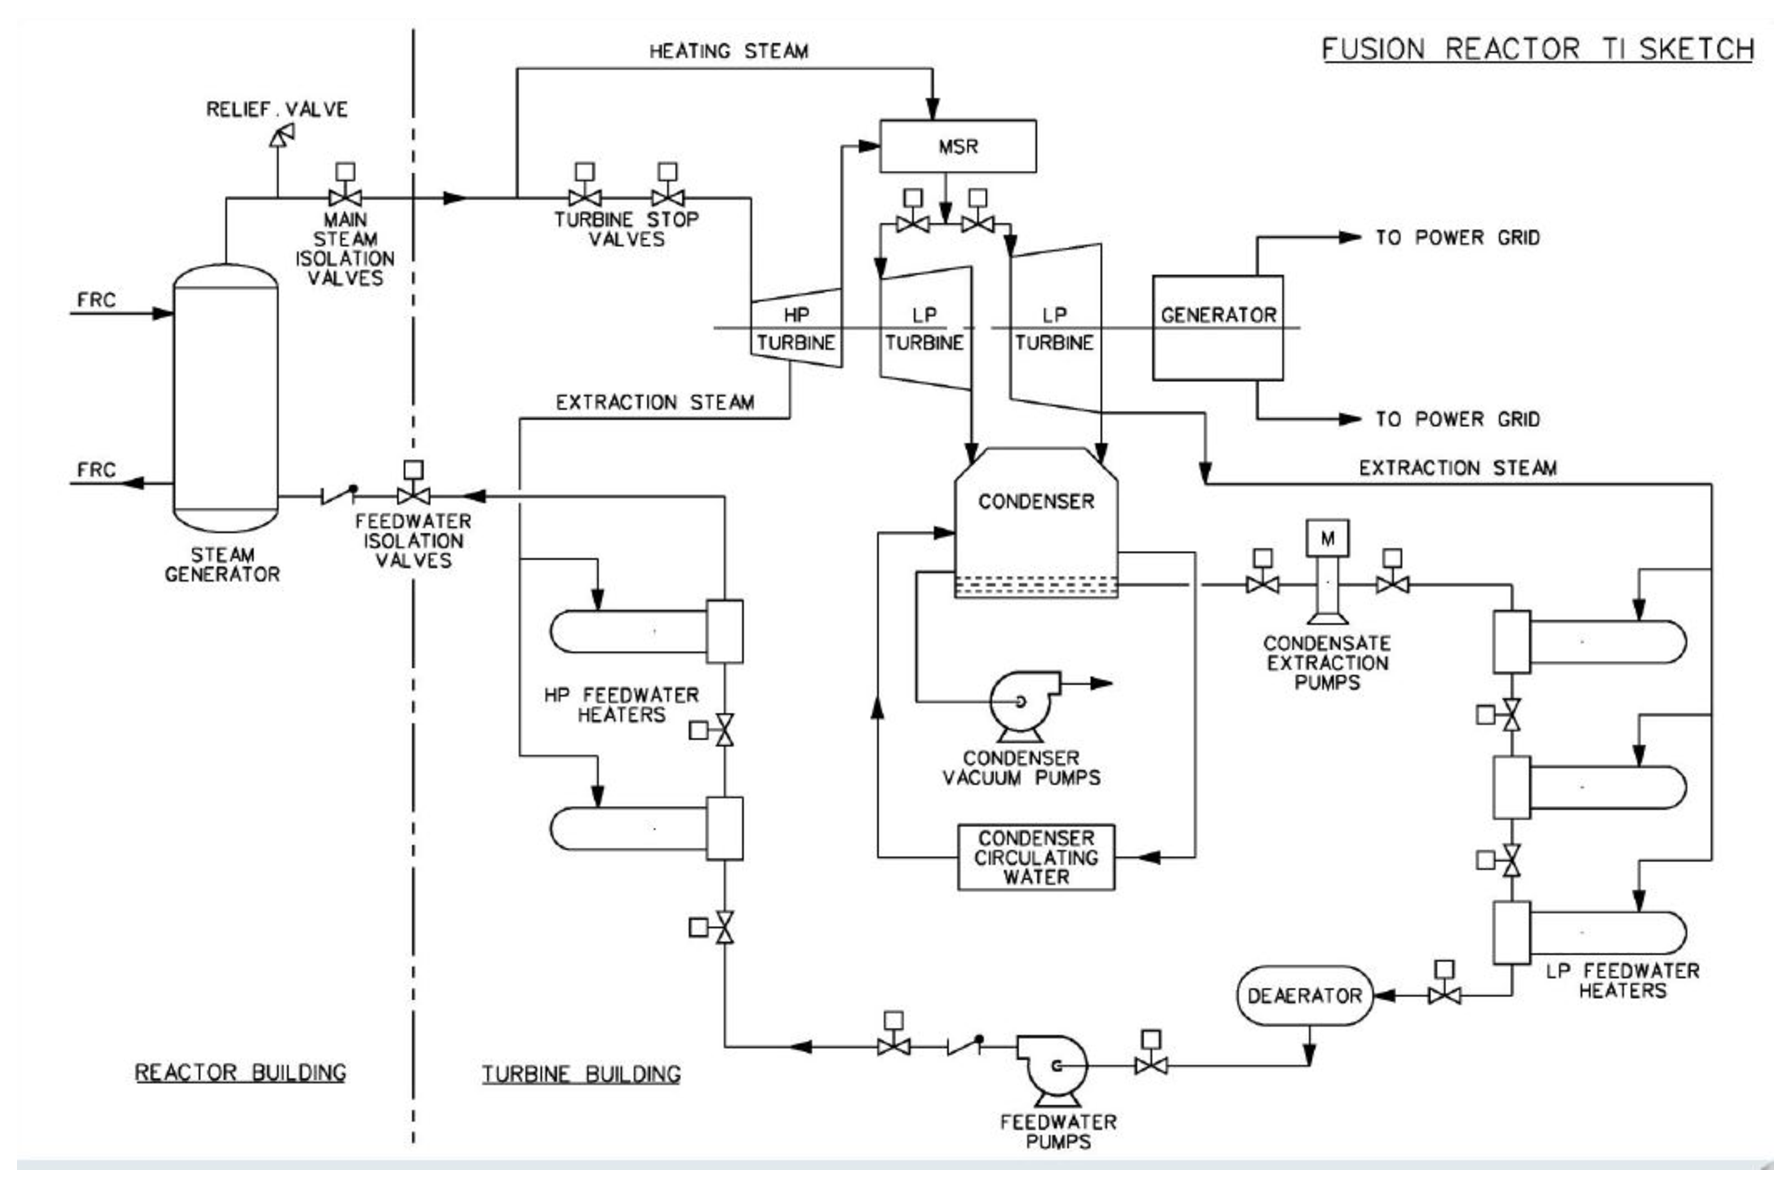
\includegraphics[scale=0.5]{StandardFigures/TIsketch.eps}   
\caption{Turbine island, per the 2017 ARPA-E study \cite{Bechtel2017}.}   
\label{fig:ti}   
\end{figure}   

Turbine Generator Equipment: This category assumes that electricity is the primary product. The categories below apply mostly to a steam-driven turbine; however, similar categories would exist for gas-driven turbines. This account includes all process equipment and systems associated with the plant output.

\begin{itemize}
    \item Cost Category 23.10.00 Turbine Generator(s): Includes turbine generator plus associated mountings, main steam control and isolation valves, lubrication system, gas systems, moisture separator, and drain system, excitation system, and controls. Main steam piping is in Account 22.20.00.
    \item Cost Category 23.30.00 Condensing Systems: Includes condenser equipment, the condensate system, the gas removal system, the turbine bypass system, condenser-cleaning system, and piping from condenser to the feedwater heating system (Cost Category 23.40.00). Condensate polishing is in Account 23.5.
    \item Cost Category 23.30.00 Feed Heating Systems: Includes the feed heating system, feedwater heaters, feedwater system piping, the extraction steam system, and the feedwater heater vent and drain system. Piping to the steam generator continues with Cost Category 22.20.00.
    \item Cost Category 23.50.00 Other Turbine Plant Equipment: Includes piping system, turbine auxiliaries, closed cooling water system, demineralized water make-up system, chemical treatment system, and neutralization system. The cooling towers are in Cost Category 26.00.00.
    \item Cost Category 23.60.00 Instrumentation and Control (I\&C): Includes turbine generator control equipment, process computer, and BOP I\&C, including software, tubing, and fittings. Cables are in Cost Category 24.6.
    \item Cost Category 23.70.00Turbine Plant Miscellaneous Items: Includes painting, welder qualification, and turbine plant insulation.
\end{itemize}

Cost basis is NETL baseline Case B12A, Cost Category 8: Steam Turbine and Accessories Bare erected cost excluding engineering, construction management, and  
contingency \$150 million in source table for Coal Plant / 686 MW electric capacity in source table = \$219/kW applied to gross thermal power, to give a total of \$ C230000 M.